\subsection{Представление слов}
\label{section:textRepsesentation}

То, как модели видят данные отличается от того, как из видят люди. Например, мы легко можем понять
предложение <<Да будет свет>>, но модели не могут --- им нужны векторы с признаками. Такие векторы являются
представлениями слов, которые может обработать наша модель.

\bigskip
Самой простой формой представления слов является дискретное представление, т.е. one-hot представление: все
слова представляются в виде вектора, размерность которого совпадает с числом слов словаре. Причем все
компоненты кроме $i$-го равны нулю, а позиция, соответствующая $i$-му слову равна единице. Очевидно, что такой
способ не самый лучший. Во-первых такое представление зависит от положения слов в словаре, а это нежелательно,
потому что задает бессмысленные отношения между словами. Во-вторых размеры такого словаря растут прямо
пропорционально количеству слов в нем, а это значит размерность его может доходить до сотен тысяч и работать с
ними станет очень вычислительно накладно. В-третьих такое представление совершенно не учитывает значение слов,
для решения этой проблемы обратимся к дистрибутивной семантике.

\subsubsection{Дистрибутивная семантика}

Чтобы зафиксировать значение слов в их векторах, нам сначала нужно определить понятие значения, которое можно использовать на практике. Для этого давайте попробуем понять, как мы, люди, узнаем, какие слова имеют схожее значение \cite{LenaVoita}.

\bigskip
Как только мы видим, как неизвестное слово используется в разных контекстах, мы в состоянии понять его значение. Гипотеза состоит в том, что мозг искал другие слова, которые можно использовать в тех же контекстах, нашел некоторые и пришел к выводу, что неизвестное слово имеет значение, подобное этим другим словам. Это гипотеза распределения:

\begin{proposition}
 Слова, которые часто встречаются в схожих контекстах, имеют одинаковое значение.
\end{proposition}

Это чрезвычайно ценная идея, ее можно использовать на практике, чтобы слова-векторы передавали их значение. Согласно гипотезе распределения, <<улавливать смысл>> и <<улавливать контексты>> по своей сути одно и то же. Следовательно, все, что нам нужно сделать, это поместить информацию о контекстах слов в представление слов. В этой части работы мы разберем два способа, как сделать это.


\subsubsection{Основная идея архитектуры нейронных сетей}

Чтобы объяснить работу нейронных сетей нужно определить из чего они состоят. Для этого рассмотрим простейший линейный бинарный классификатор -- перцептрон Розенблата. Пространство данных разделяется на два множества гиперплоскостью, а метка класса будет ставиться в зависимости от значения линейной функции от входных признаков.

\begin{equation}
 \sign (w_0 + w_1x_1 + w_2x_2 + \ldots + w_dx_d),
\end{equation}

где $x =(x_1, x_2, \ldots, x_d) \in \mathds{R}^d$. Мы ищем такие веса $w_0, w_1 \ldots, w_d \in \mathds{R}^d$, чтобы $\sign$ от скалярного произведения признаков и весов $w^\top x$ совпадал с верной меткой $y(x) \in {-1,1}$, но для этого добавим фиктивную переменную в вектор $x =(1, x_1, x_2, \ldots, x_d) \in \mathds{R}^{d+1}$, чтобы размерности сохранялись.

\bigskip
Теперь обучим эту функцию, для этого нам нужна функция ошибки, она называется критерий Перцептрона:

\begin{equation}
 L_P(w) = - \sum_{x \in M} y(x)(w^\top x),
\end{equation}

где $M$ --- множество неверно классифицируемых примеров. В качестве оптимизатора выберем градиентный спуск. С помощью него мы минимизируем суммарное отклонение предсказаний классификатора от верных, но только в неправильную сторону. Верное предсказание никак не влияет на функцию ошибки. В результате получается кусочно-линейная функция, которая почти везде дифференцируема и этого достаточно для применения градиентного спуска. Процесс обучение выглядит так: если предсказание верное, то не делаем ничего, если классификатор ошибся, то делаем градиентный шаг.

\bigskip
Такая модель перцептрона линейная и результат ее работы не слишком содержателен. Чтобы из перцептронов можно
было составить сеть, нужно добавить нелинейность. Такой нелинейностью будет функция активации. Они бывают
разные, самая распространенная --- сигмоида рис. \ref{fig:sigmoid}, она позволяет моделировать вероятность:

\begin{equation} \label{eq:sigma}
    \sigma (x) = \frac{1}{1+e^{-x}}
\end{equation}

\begin{figure}[ht]
    \centering
    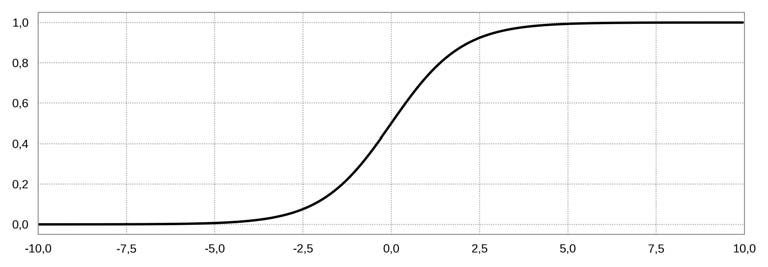
\includegraphics[scale=0.8]{sigmoid.png}
    \caption{Сигмоида}
    \label{fig:sigmoid}
\end{figure}

Обучить этот перцептрон также не составляет труда. Просто теперь мы будем решать задачу бинарной
классификации, а функция ошибки будет cross-энтропией:

\begin{equation}
 L(w) = -\frac{1}{N}\sum_{i=1}^N(y_i\log\sigma(w^\top x_i) + (1-y_i)\log(1-\sigma(w^\top x_i))).
\end{equation}

Эта функция дифференцируема, значит мы можем сделать градиентный шаг. При этом прецептрон с сигмоидой
реализует логистическую регрессию. Обобщение этой модели можно найти в разделе \ref{subsection:logreg}.

\bigskip
Графическое изображение структуры перцептрона представлено на рис. \ref{fig:neuron}, \textit{a}.

\begin{figure}[ht]
    \centering
    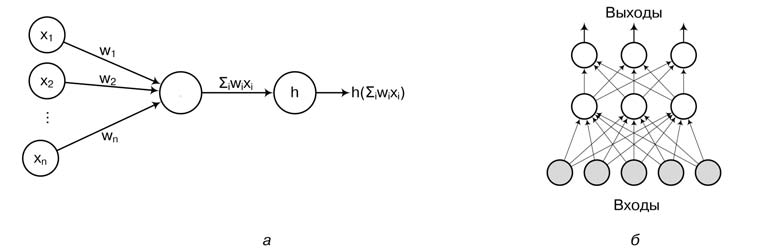
\includegraphics[scale=0.8]{neuron.png}
    \caption{(a) граф вычислений перцептрона; (б) полносвязная нейронная сеть с одним скрытым слоем.}
    \label{fig:neuron}
\end{figure}

На  рис. \ref{fig:neuron}, \textit{б} изображена несложная нейронная сеть, на ее примере покажем как можно векторизовать вычисления в слое нейронов с применением функции активации.

\bigskip
Пусть у нас в слое $k$ нейронов с весами $w_1, w_2, \ldots, w_k$, $\quad w_i = (w_{i1}, \ldots, w_{in})^\top$, на вход вектор $x = (x_1, x_2, \ldots, x_n)^\top$. В результате получим выход $y_i = f(w_i^\top x)$, где $f$ --- функция активации. Эти вычисления можно представить в векторной форме:

\begin{equation*}
\begin{pmatrix}
   y_1 \\
   \ldots \\
   y_k
\end{pmatrix} = y = f(Wx) =
\begin{pmatrix}
   f(w_1^\top x)\\
   \ldots \\
   f(w_k^\top x)
\end{pmatrix}\text{, где } W =
\begin{pmatrix}
   w_1 \\
   \ldots \\
   w_k
\end{pmatrix} =
\begin{pmatrix}
   w_{11} & \ldots & w_{1n}\\
   \ldots &  & \ldots\\
   w_{kk} & \ldots & w_{kn}\\
\end{pmatrix}.
\end{equation*}


% \subsubsection{Функции активации}

Обычно в нелинейных неронах применяется сигмоида (\ref{eq:sigma}), о которой писалось выше. Но существуют и другие функции активации, например, SoftMax или нормализованная экспонента. Она нужна чтобы обобщить функцию ошибки для задач классификации, где классов больше 2-х. Ее удобно использовать на последних слоях нейронной сети, чтобы моделировать из выхода вероятность.

% $\text{ReLU} = max(0, x)$. Чтобы понять, как она появилась рассмотрим сумму бесконечного ряда сигмоид, каждая из которых смещена на единицу относительно предыдущей:

% \begin{equation*}
%  f(x) = \sigma(x+\frac{1}{2} + \sigma(x-\frac{1}{2} + \sigma(x-\frac{3}{2}) + \ldots
% \end{equation*}
%
% $f(x)$ можно представить в виде интегала:
%
% \begin{equation*}
%  \int_\frac{1}{2}^\infty \sigma(x+\frac{1}{2}-y)dy,
% \end{equation*}
%
% Его значение можно приблизить единичными прямоугольниками:
%
% \begin{equation*}
% \begin{aligned}
%   \sum_{i=0}^\infty \sigma(x+\frac{1}{2}-i) & \approx \int_\frac{1}{2}^\infty \sigma(x+\frac{1}{2}-y)dy = \\
%   & = \left[-\log (1+e^{x+\frac{1}{2}-y})\right]^{y=\infty}_{y=\frac{1}{2}} = \log (1+e^x),
% \end{aligned}
% \end{equation*}
%
% а это в точности интеграл от сигмиоды:
%
% \begin{equation*}
%  \int \sigma (x) dx = \log(1+e^x) + C.
% \end{equation*}
%
% Получается бесконечный ряд сигмоид гораздо более выразительная функция активации и это почти тоже самое что и
% $\log(1+e^x)$



% Это приближение к ф-ии log(1+e^x) (SoftPlus), которая получается из суммы бесконечного ряда сигмоид со смещением на 1/2 и тд. Это дает возможность отличать сильно активированные нейроны от слабо активированных. Но считать производную такой функции очень накладно, поэтому ее приближение -- хороший компромисс. Существуют еще разные модификации ReLU, например, PReLU или LReLU. В целом она показала лучшую эффективность по сравнению с сигмоидой и tanh, следовательно используется повсеместно.
%










































\subsubsection{Распределенные представления слов word2vec}

Подход к обучению моделей распределенных представлений слов был описан в работе Йошуа Бенджи с соавторами
\cite{Bengio}, которая была продолжена в \cite{Zhou}. Идея подхода описанного в \cite{Bengio} основанна на
задаче построения языковой модели, процесс обучения выглядит так:

\bigskip
\begin{itemize}
 \item всем токенам из словаря $i \in V$ ставят в соответствие вектор признаков $w_i$ размерности $d$ ($w_i
\in \mathds{R}^d$). Стандартным значением $d$ является 300;

 \item теперь можно определить вероятности для каждого токена $i$, что он появится в контексте $c_1, \ldots,
c_n$. Для этого определим функцию от векторов признаков $w$:

 \begin{equation}
  \hat{p}(i|c_1, \ldots, c_n) = f(w_i, w_{c_1}, \ldots, w_{c_n}; \theta),
 \end{equation}

 где $w_{c_1}, \ldots, w_{c_n}$ --- векторы признаков токенов из контекста, a $f$ --- фунция с параметрами
$\theta$, которая принимает векторы признаков;

 \item максимизируя логарифм правдоподобия большого корпуса текстов можно обучить векторы признаков $w$ и
параметры $\theta$

 \begin{equation}
  L(W, \theta) = \frac{1}{K}\sum_t \log{f(w_k, w_{k-1}, \ldots, w_{k-n+1}; \theta) + R(W, \theta)},
 \end{equation}

 где $K$ размер окна контекста, а $R(W, \theta)$ --- регуляризация.

\end{itemize}

\bigskip
Для получения функции $f$ можно использовать нейронную сеть. Модель word2vec строится на описании
нейросетевой модели, предложенной в \cite{Bengio}. Она была разработана Томасом Миколовым с соавторами и
опубликована в работах \cite{Mikolov:1, Mikolov:2}, причем в двух вариациях:

\bigskip
\begin{itemize}
 \item CBOW (Continious Bag Of Words) --- по контексту восстановить слово;
 \item skip-gram --- восстановить контекст в зависимости от слова;
\end{itemize}

\bigskip
Архитектура word2vec представляет собой полносвязную нейронную сеть с одним скрытым слоем рис.
\ref{fig:word2vec}.

\begin{figure}[ht]
    \centering
    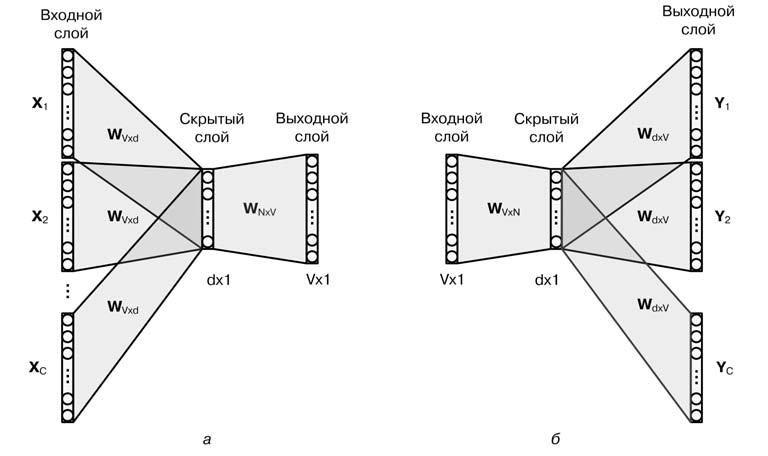
\includegraphics[scale=0.8]{word2vec.png}
    \caption{(a) CBOW; (б) skip-gram.}
    \label{fig:word2vec}
\end{figure}

% !! смещение
Принцип работы модели CBOW \cite{Nikolenko} рис. \ref{fig:word2vec}, \textit{а}  выглядит так:

\bigskip
\begin{itemize}
 \item на вход сети подаются one-hot вектора размерности $V$, где V --- это размер словаря;
 \item скрытый слой --- это матрица $W$ размерности $V\times d$, которая переводит наши представления слов в
$d$ - мерное пространство;
 \item на выходе для каждого слова в словаре берем среднее всех полученных векторов и получаем оценку $u_j$,
где $j = 1, \ldots, V$.
\end{itemize}

\bigskip
Чтобы найти апострериорное распределение модели, просто вычисляем softmax:

\begin{equation}
 \hat{p}(i|c_1, \ldots, c_n) = \frac{\exp{u_j}}{\sum_{j'=1}^V \exp{u_{j'}}}.
\end{equation}

Для аппроксимации апостериорным распределением распределения данных используем loss-функцию для одного окна:

\begin{equation}
 L = -\log{p(i|c_1, \ldots, c_n)} = - u_j + \log{\sum_{j'=1}^{V} \exp{u_{j'}}}.
\end{equation}

Принцип работы модели skip-gram рис. \ref{fig:word2vec}, \textit{б} полностью противоположный. До этого мы
усредняли контекст, чтобы получить среднее слово в окне, а теперь будем предсказывать слова контекста исходя
из центрального слова. На выходе мы получаем $K-1$ мультиномиальных распределений (центральное слово не
учитывается):

\begin{equation}
 \hat{p}(c_k|i) = \frac{\exp{u_{kc_k}}}{\sum_{j'=1}^V \exp{u_{j'}}},
\end{equation}

loss-функция для окна размера K выглядит так:

\begin{equation}
 L = -\log{p(c_1, \ldots, c_n|i)} = - \sum_{k=1}^{K} u_{kc_k} + n\log{\sum_{j'=1}^{V} \exp{u_{j'}}}.
\end{equation}

Возникает вопрос, как же обучить такую модель? Этот процесс хорошо описан в докладе Голдберга и его соавторов
\cite{Goldberg}.

\bigskip
Подробно разберем модель skip-gram для корпуса документов $D$. Нашей задачей стоит нахождение оптимальных
параметров модели $\theta$, чтобы максимизировать функцию правдоподобия:

\begin{equation} \label{eq:likelyhood}
 L(\theta)=\prod_{i\in D}\left(\prod_{c\in C(i)} p(c|i;\theta)\right) = \prod_{(i,c)\in D}p(c|i;\theta),
\end{equation}

где $C(i)$ --- множество контекстных слов внутри окна вокруг центрального слова $i$. Вероятность $p(c|i;\theta
)$ определяется, как softmax-функция, зависящая от всех возможных векторов контекста.

\begin{equation} \label{eq:generalSoftmax}
 p(c|i;\theta) = \frac{\exp{\tilde{w}_c^\top w_i}}{\sum_{c'} \exp{\tilde{w}_{c'}^\top w_i}},
\end{equation}

где $\tilde{w}_c$ --- вектор признаков слова из контекста $c$, который отличается от $w_i$. Для каждого слова
$i$ надо обучить два вектора признаков $w_i$ и $\tilde{w}_i$, в первом случае это слова выступает в качестве
центрального, во втором в качестве контекстного.

\bigskip
Эта особенность обучения, когда мы берем два разных вектора одного и того же слова вместо одного, описана в
\cite{Goldberg}. И мотивирована тем, что слова редко встречаются в контексте себя самих. Вот, например, слово
<<мотивация>> вряд ли можно встретить в контексте другого слова <<мотивация>>, под это правило попадают почти
все слова. Поэтому в процессе обучения модель сведет вероятности $p(i|i, \theta)$ к нулю. А если вектора
контекста и центрального слова будут равны нулю, то норма вектора $|w_i| = w_i^\top w_i$ тоже будет равняться
нулю, а это очень не желательно. Поэтому для каждого слова мы обучаем два разных вектора.

\bigskip
Теперь выразим максимум функции правдоподобия для всего корпуса через логарифм (\ref{eq:likelyhood}) и
(\ref{eq:generalSoftmax}):

\begin{equation}
\begin{aligned}
 \argmax_{\theta} \prod_{(i,c)\in D} & p(c|i;\theta) = \argmax_{\theta} \sum_{(i,c)\in D}\log{p(c|i;\theta)} =
\\
 & = \argmax_{\theta} \sum_{(i,c)\in D} \left(\exp{\tilde{w}_c^\top w_i} - \log{\sum_{c'}
\exp{\tilde{w}_{c'}^\top w_i}}\right).
\end{aligned}
\end{equation}

Оптимизируя данную функцию мы получаем хорошее распределенное представление слов. Но для этого нужно решить
сложнейшую задачу: суммировать скалярные произведения всех возможных слов и их контекста $\sum_{c'}
\tilde{w}_c^\top w_i$ при том, что размер словаря может достигать миллионов.

\bigskip
Чтобы уменьшить количество вычислений Миколов с соавторами \cite{Mikolov:2} предложили элегантный метод:
negative sampling. Нам не нужно считать всю сумму $\sum_{c'} \tilde{w}_c^\top w_i$, а только случайно выбрать
несколько ее элементов в качестве отрицательных примеров (примеры в которых слово не находится в определенном
контексте) и обновить только их. Т.е. теперь нам нужно посчитать только небольшую сумму $\sum_{c' \in D'}
\tilde{w}_c^\top w_i$, где $D'$ --- случайное подмножество отрицательных примеров.

\bigskip
По сути negative sampling --- это тоже правдоподобие, но другого события. Пусть у нас есть слово $i$ и его
контекст $c$, наша задача максимизировать вероятность $p((i,c) \in D; \theta)$, параметризированную вектором
$\theta$, т.е. правдоподобие появления пары $(i,c)$:

\begin{equation}
 \argmax_{\theta} \prod_{(i,c)\in D} p((i,c)\in D;\theta) = \argmax_{\theta} \sum_{(i,c)\in D} \log{
p((i,c)\in D;\theta)}.
\end{equation}

Выразим $p((i,c)\in D;\theta)$ через softmax. Но так как это бинарное событие, то заменим softmax сигмоидой
$\sigma (x) = \frac{1}{1+\exp{(-x)}}$:

\begin{equation}
 p((i,c)\in D;\theta) = \frac{1}{1+\exp{(-\tilde{w}_c^{\top} w_i)}}
\end{equation}

Максимизируем логарифм правдоподобия:

\begin{equation} \label{eq:negLikelyhood}
\begin{aligned}
 \argmax_{\theta} \sum_{(i,c)\in D} & \log{p((i,c)\in D;\theta)} = \\
 & = \argmax_{\theta} \sum_{(i,c)\in D} \log{\frac{1}{1+\exp{(-\tilde{w}_c^{\top} w_i)}}}.
\end{aligned}
\end{equation}

Из (\ref{eq:negLikelyhood}) видно, что оптимальное значение логарифма будет получено при максимальном значении
скалярного произведения $\tilde{w}_c^{\top} w_i$. Сделаем равные векторы с большой нормой и можно без проблем
получить правдоподобие почти равное единице. Подвох заключается в том, что модель обучается на данных для
бинарной классификации, но мы рассматриваем только набор состоящий из положительных примеров. Классификатор,
который всегда предсказывает <<да>> --- плохой. Поэтому имеет смысл добавить отрицательных примеров, просто
случайно выбирая слова и контекст, которых нет в данных. После того, как мы получим набор отрицательных
данных, максимизация правдоподобия будет выглядеть так:

\begin{equation} \label{eq:generalLikelyhood}
 \argmax_{\theta} \prod_{(i,c)\in D} p((i,c)\in D;\theta) \prod_{(i,c)\in D'} p((i',c')\notin D;\theta)
\end{equation}

Выразим в (\ref{eq:generalLikelyhood}) пару $(i,c) \in D$:

\begin{equation}
\begin{aligned}
 & \argmax_{\theta} \prod_{(i,c)\in D} p((i,c)\in D;\theta) \prod_{(i,c)\in D'} 1-p((i',c')\in D;\theta) = \\
 = & \argmax_{\theta} \left[\sum_{(i,c)\in D} \log{p((i,c)\in D;\theta)} + \sum_{(i,c)\in D'} \log{(
1-p((i',c')\in D;\theta))} \right] = \\
 = & \argmax_{\theta} \sum_{(i,c)\in D} \left[\log{\frac{1}{1+\exp{(-\tilde{w}_c^{\top} w_i)}}} +
\sum_{(i,c')\in D'} \log{\frac{1}{1+\exp{(\tilde{w}_{c'}^{\top} w_i)}}} \right] = \\
 = & \argmax_{\theta} \sum_{(i,c)\in D} \left[\log\sigma(\tilde{w}_c^{\top} w_i) + \sum_{(i,c')\in D'}
\log\sigma(-\tilde{w}_{c'}^{\top} w_i)\right]
\end{aligned}
\end{equation}

Получили формулу для negative sampling из \cite{Mikolov:2}. Значит мы для каждого окна случайно берем
несколько отрицательных примеров $D'$ и делаем градиентный шаг для loss-функции:

\begin{equation}
 L = \log\sigma(\tilde{w}_c^{\top} w_i) \sum_{(i,c')\in D'} \log\sigma(-\tilde{w}_{c'}^{\top} w_i)
\end{equation}

Аналогичные рассуждения можно провести для модели CBOW.

% ++ можно добавить матричный подход

\subsubsection{ELMo}

Создание этой модели породило новую эру распределенных представлений слов. Word2vec показал, что с помощью векторов можно представлять слова в виде, который может передавать их семантику или смысловые отношения (т.е. способность различать схожие и противоположные по смыслу слова или находить параллели в отношениях таких словарных пар, как <<Женщина - Мама>> и <<Транспорт - Повозка>>), а также синтаксические или грамматические отношения (например, определять, что отношение между <<Красиво и Красивый>>) \cite{elmoru}.

\bigskip
Почему бы не сделать распределенное представление слов на основе контекста, в котором оно стоит? Чтобы передавать не только значение слова, но и контекстуальную информацию. Так появились контекстуализированные распределенные представления слов (contextualized word-embeddings)

\bigskip
Способность понимать язык ELMo получила после обучения предсказыванию нового слова в последовательности слов. Эта задача, называется языковым моделированием (language modeling).

\bigskip
В \cite{elmoen} показано, что двунаправленная языковая модель (biLM) является основой для ELMo. В то время как входные данные представляют собой последовательность $n$ слов $(x_1, \ldots, x_n)$ языковая модель предсказывает условную вероятность следующего слова:

\bigskip
В прямом проходе последовательность содержит слова перед целевым словом:

\begin{equation*}
  p(x_1, \ldots, x_n) = \prod_{i=1}^n p(x_i| x_1, \ldots, x_{i-1}).
\end{equation*}

\bigskip
При обратном проходе последовательность содержит слова после целевого слова:

\begin{equation*}
  p(x_1, \ldots, x_n) = \prod_{i=1}^n p(x_i| x_{i+1}, \ldots, x_n).
 \end{equation*}

\bigskip
Предсказания в обоих направлениях моделируются многослойными LSTM ячейками со скрытыми состояниями $\overrightarrow{h}_{i,l}$ и $\overleftarrow{h}_{i,l}$ и для входного слова $x_i$ на уровне слоя $l = 1, \ldots, L$. Скрытое состояние последнего слоя $h_{i,L} = [\overrightarrow{h}_{i,L}; \overleftarrow{h}_{i,L}$ используется для вывода вероятностей по словам после нормализации softmax. Эти скрытые состояния разделяют слой распределенного представления слов и слой softmax, которые параметризованы $\Theta_e$ и $\Theta_s$ соответственно.

\begin{figure}[ht]
    \centering
    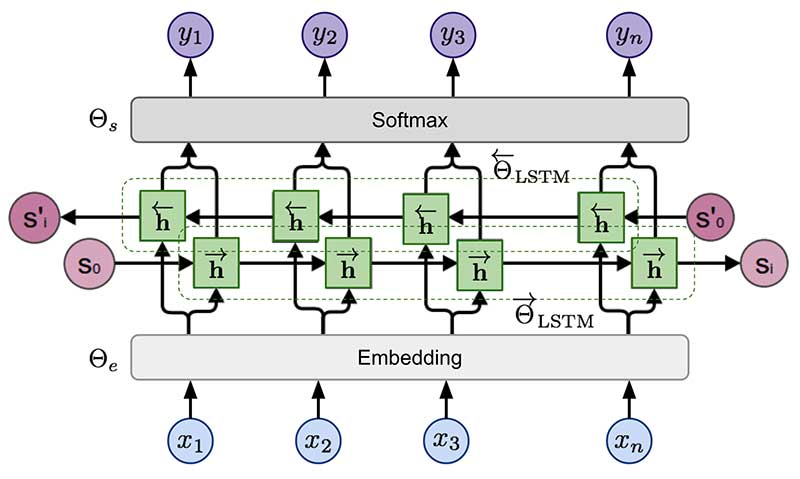
\includegraphics[scale=0.5]{ELMo.jpg}
    \caption{Базовая модель biLSTM ELMo. Источник: \cite{elmopic}}
    \label{fig:elmo}
\end{figure}

\bigskip
Процесс обучения модели --- максимизация логарифма правдоподобия для истиных слов в обоих направлениях:

\begin{equation*}
\begin{aligned}
 \lh (x) = \argmax \sum_{i=1}^n \bigg[ & \log p(x_i| x_1, \ldots, x_{i-1}|\Theta_e,\overrightarrow{\Theta}_{LSTM}, \Theta_s) + \\
 + & \log p(x_i| x_{i+1}, \ldots, x_n| \Theta_e,\overleftarrow{\Theta}_{LSTM}, \Theta_s)\bigg]
\end{aligned}
\end{equation*}






